\section{Arquitectura}

En la Figura \ref{fig:ids_sensor} puede observar un esquema del proceso por el cual el sistema se sometería al estar en funcionamiento. La descripción del proceso es el que se especifica debajo de la figura.\\


% \begin{figure}
% 	\centering
% 	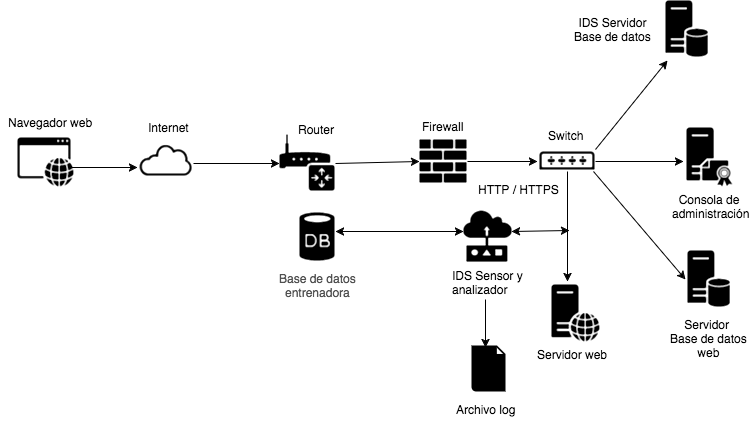
\includegraphics[scale=.6]{images/Diagrama_general_de_despliegue}
% 	\caption{Esquema de la arquitectura a implementar.}
% 	\label{fig:arqui_IDS}
% \end{figure}

\begin{figure}
	\centering
	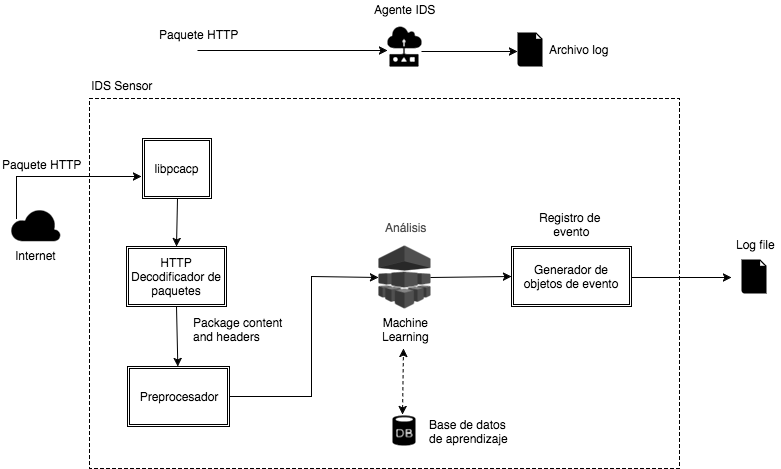
\includegraphics[scale=.6]{images/IDS_Sensor}
	\caption{Esquema de la arquitectura a implementar.}
	\label{fig:ids_sensor}
\end{figure}

El ataque XSS será ejecutado sobre una página web vulnerable. Al llegar el ataque al servidor, el tráfico generado por este será analizado dentro del mismo por el agente.\\

Al ser detectado el ataque, el agente envía los datos del ataque al servidor administrador.\\

El servidor administrador registra el evento en una base de datos y envía las notificaciones del ataque. La primera notificación será en la interfaz de monitoreo del sistema y la otra notificación se enviará a las cuentas configuradas de SMS y correo electrónico del administrador encargado.\\

El evento será almacenado en una base de datos para su posterior análisis por el administrador encargado.\\

El administrador recibirá las notificaciones correspondientes por parte del sistema con la información necesaria del evento.\\

El administrador una vez notificado, podrá ver los registros de los eventos ocurridos para tomar las medidas necesarias a la seguridad de sus aplicaciones web.\\

%A futuro se espera que el sistema pueda ser escalable haciendo un sistema más robusto para la detección de ataques XSS e inclusive se pueda agregar módulos para una mayor cobertura de ataques.

\begin{figure}
	\centering
	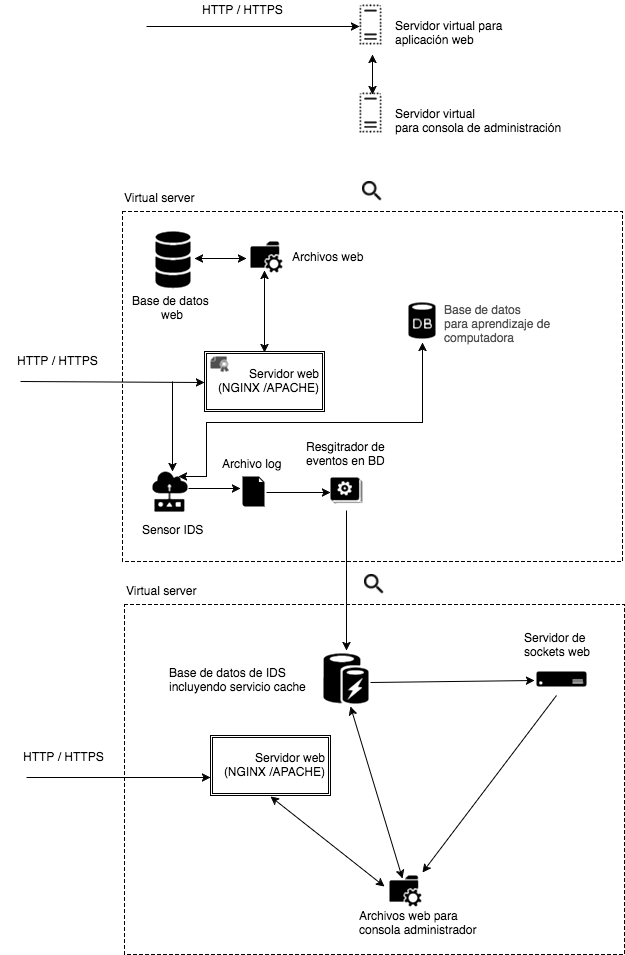
\includegraphics[scale=.6]{images/Diagrama_de_despliegue_1_server}
	\caption{Diagrama de arquitectura ideal de interacción de módulos.}
	\label{fig:arqui_server}
\end{figure}

En el diagrama \ref{fig:arqui_server} se puede observar la estructura ideal y la interconexión de los componentes del IDS. El cual comienza con un \textit{request} al servidor host cuyo paquete es interceptado por el agente antes de que llegue el servidor web, su labor será (mediante machine learning) determinar el riesgo del paquete. A la salida del agente cada evento se guardará en un archivo log por día. \\

\begin{figure}
	\centering
	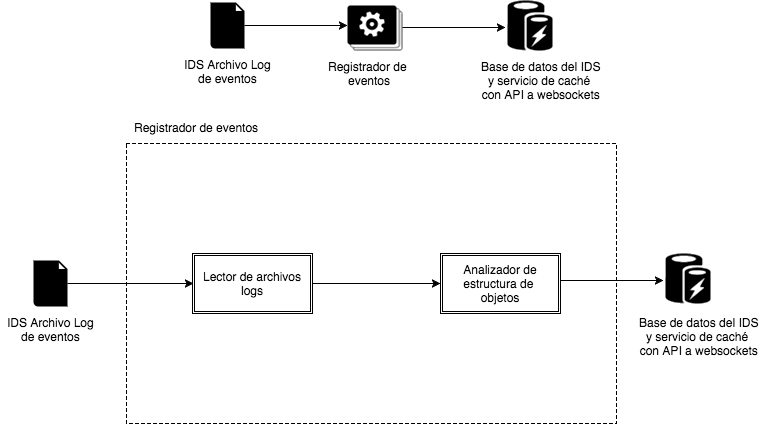
\includegraphics[scale=.6]{images/Worker}
	\caption{Diagrama de componentes para el registrador de eventos.}
	\label{fig:ids_worker}
\end{figure}

El diagrama \ref{fig:ids_worker} corresponde al registrador de eventos, cuyo labor es leer los archivos \textit{logs} generados por el agente, analizar la correcta estructura de los eventos en este archivo y guardarlos en un servidor de base de datos ya sea local o remoto. Además es el encargado de convertir los archivos \textit{logs} en registros de la base de datos y de registrar dichos eventos en un servidor de estructuras de datos o también conocido como servicio de caché que le permitira a un servidor de websockets cachar cada nuevo registro en este almacén de datos y ofrecerlo en algún canal socket configurado. \\

En entornos en los que un IDS tenga que procesar una gran cantidad de tráfico es muy posible que su rendimiento se vea afectado y acabe descartando paquetes Esto es debido a que el IDS no procesaria el siguiente paquete hasta que no terminara de escribir el evento en la base de datos. Este proceso de escritura es lento si hablamos de que es necesario una conexión TCP y un insert en la base de datos por cada alerta. Por lo que esté modulo implementando correctamente es decir, con un eficiente uso de concurrencia permitirá al IDS liberar recursos que por ende, permitirá a nuestro agente procesar más paqeuetes de forma más rápida y eficiente. \\

\begin{figure}
	\centering
	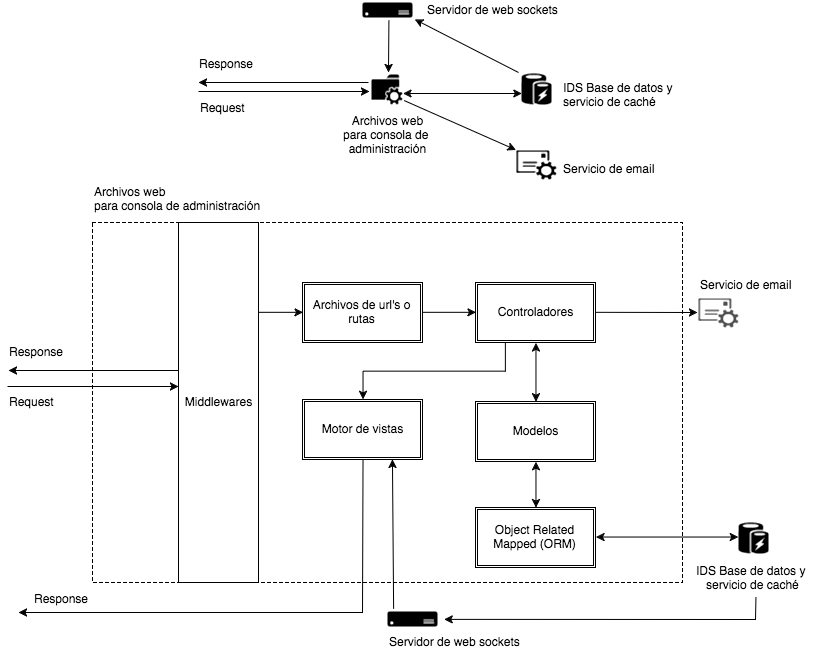
\includegraphics[scale=.6]{images/Report_Viewer}
	\caption{Diagrama de componentes para la consola de administración.}
	\label{fig:ids_report}
\end{figure}

El diagrama \ref{fig:ids_report} corresponde al diseño de la consola de administración usando el patrón MODELO-VISTA-CONTROLADOR, el cual desde el crecimiento exponencial del uso de la internet las aplicaciones cliente-servidor son la mejor opción para diseñar aplicaciones web. Ahunado a esto, los controladores del sistema se conectan a servicios de email para enviar correos cuando sean necesarios. Las vistas se conectan a un servidor de \textit{web cockets} con lo que estará recibiendo eventos en tiempo real y nos servirá para la monitorización del sistema. \\

\begin{figure}
	\centering
	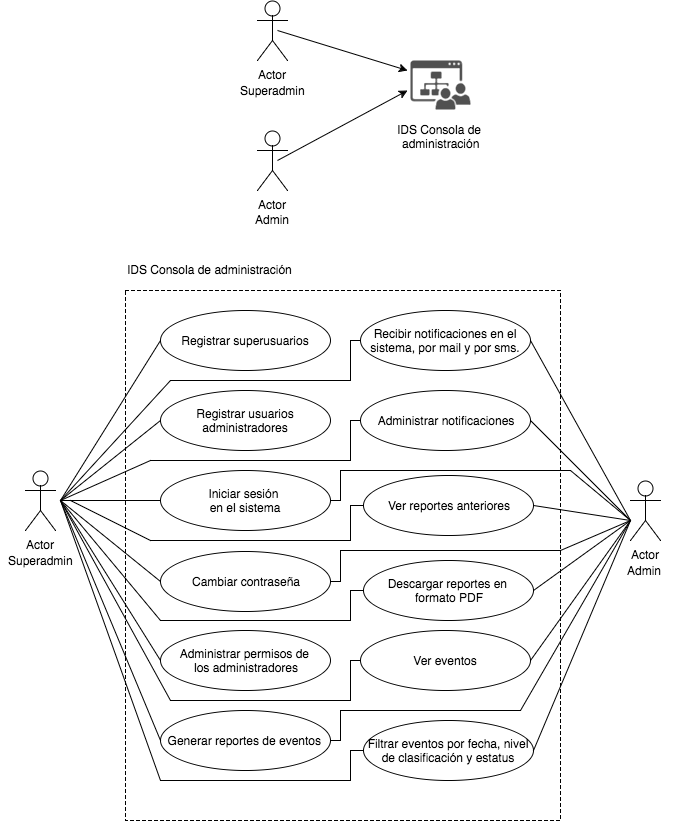
\includegraphics[scale=.6]{images/Casos_de_uso_Report_Viewer}
	\caption{Casos de uso para consola de administración.}
	\label{fig:ids_ucrv}
\end{figure}

De acuerdo a los requisitos del sistema se determinaron los casos de usos correspondientes a la consola de administración mostrados en la figura \ref{fig:ids_ucrv} con los diferentes actores que podrían interactuar con el sistema. \\

A continuación se muestran los diagramas de objetos de cada componente del sistema. La figura \ref{fig:ids_doosensor} correponde a los modelos  del agente y el registrador de eventos y la figura \ref{fig:ids_doos} correponden a los modelos para la consola de administración. \\

\begin{figure}
	\centering
	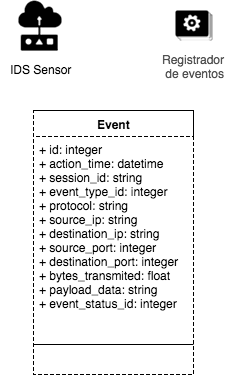
\includegraphics[scale=.6]{images/Diagrama_Objetos_Sensor_IDS}
	\caption{Diagrama de objetos para agente IDS y el registrador de eventos.}
	\label{fig:ids_doosensor}
\end{figure}

\begin{figure}
	\centering
	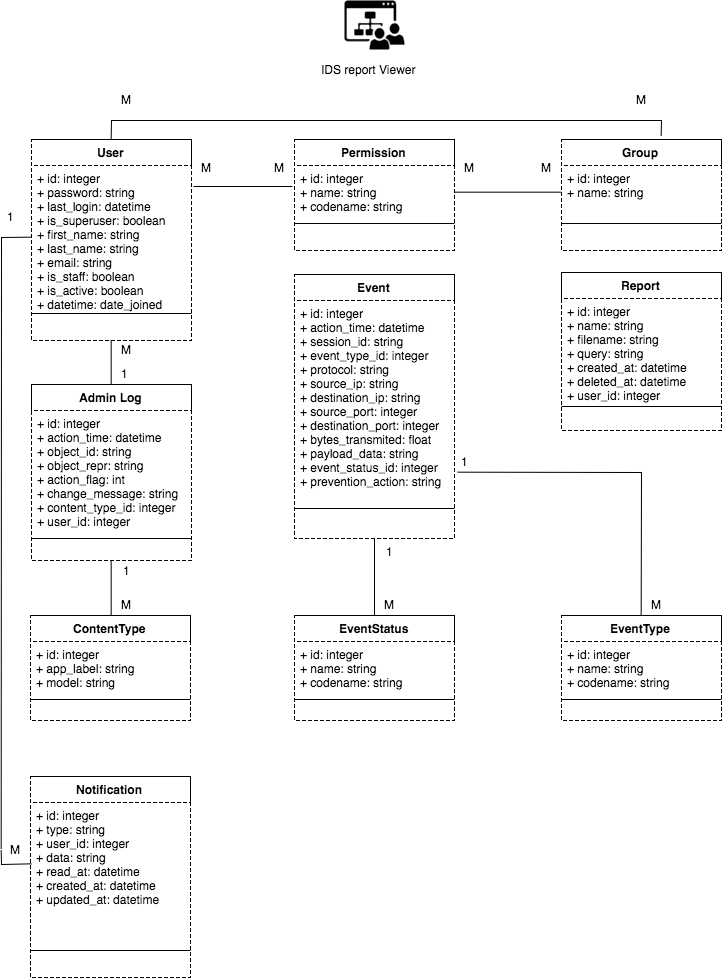
\includegraphics[scale=.6]{images/Diagrama_de_objetos}
	\caption{Diagrama de objetos para consola de administración.}
	\label{fig:ids_doos}
\end{figure}

Debido a las razones antes mencionadas en lo que corresponde a la base de datos de eventos salientes del agente. Sólo se requiere diseñar la estructura de la base de datos del registrador de eventos y la consola de administración y debido a que estos dos componentes comparten la misma instancia de almacenamiento el diagrama entidad-relación queda definido, como se observa en la figura \ref{fig:ids_er}, de acuerdo a los requisitos inciales del sistema. \\

\begin{figure}
	\centering
	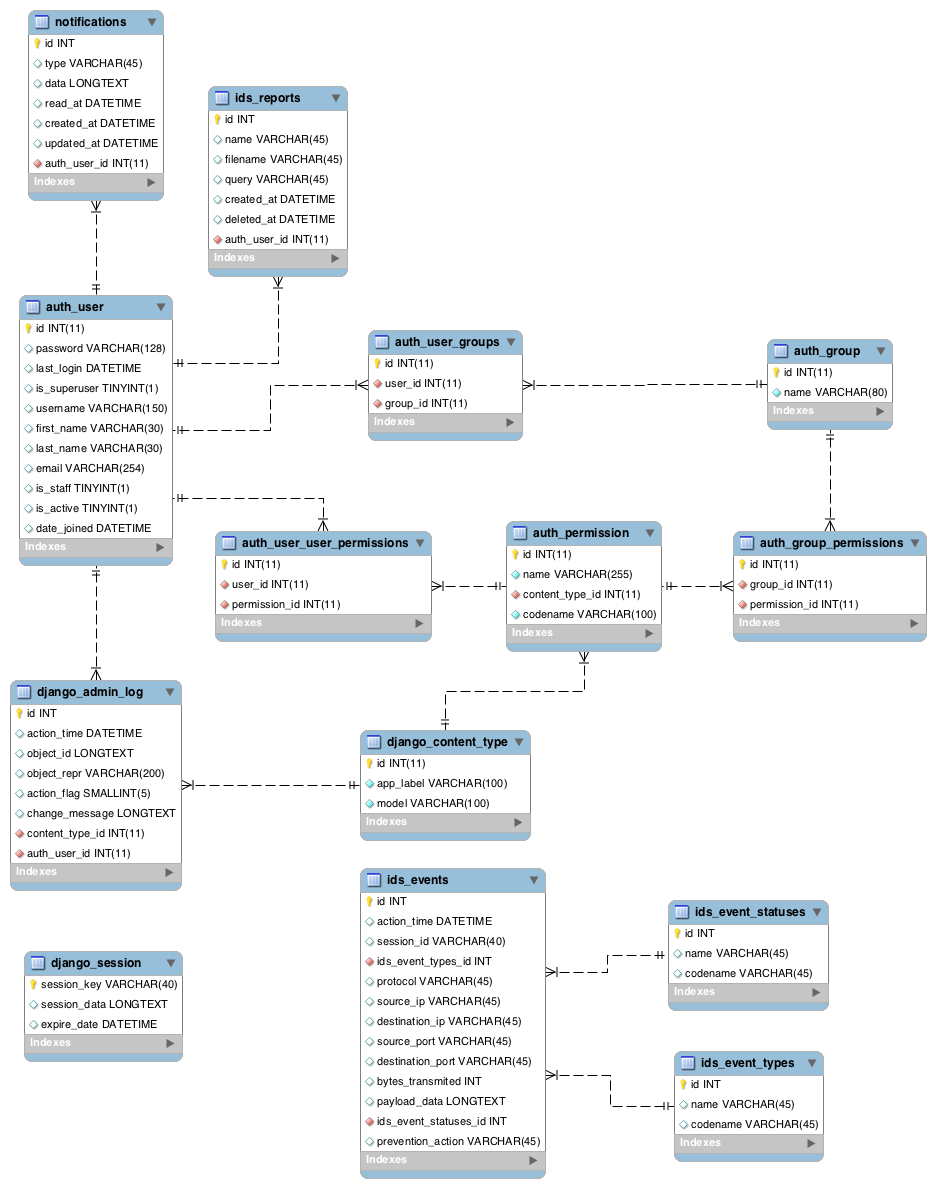
\includegraphics[scale=.4]{images/er_console_diagram}
	\caption{Diagrama entidad relación de la base de datos para guardar eventos del IDS y la consola de administración.}
	\label{fig:ids_er}
\end{figure}
